%% =====================================================================
%% NEW main-text experiment (Sarat): structured local mass at ResNet scale.
%% \input in Section 6 (Experiments), after Experiment 4. Prose in BLUE.
%% (arXiv version: main text. For a page-limited camera-ready this can move to
%%  an appendix.)
%% Round-3 (Sarat, 24 Aug 2026): added small-ball figures for CIFAR and ImageNet,
%% corrected the ImageNet caption, noted the ImageNet family coverage, and
%% replaced "dichotomy" with the correct one-sided statement.
%% =====================================================================

\paragraph{Experiment 5: Local mass at ResNet scale (structured channel gates).}
{\color{blue}
We extend Experiment~4 to \emph{structured} (channel-gate) variational posteriors on
larger networks: ResNet-56 on CIFAR-10 and ResNet-50 on ImageNet. A variational gate is
attached to each prunable channel of a pretrained network, and the gates are trained (base
frozen) under a spike-and-slab gate prior, so the measured per-channel object is the gate
value \(z\) (channel multiplier). An atom-capable gate (spike-and-slab, hard-concrete)
places an atom at \(0\), i.e.\ a channel switched off, giving \(\MI_{\mathrm{pow}}=\infty\);
a continuous gate (Gaussian, Student-\(t\)) has no atom, \(\MI_{\mathrm{pow}}=1\), and
assigns vanishing mass to the channel-off event.
\add{All four families are reported on both networks. The ImageNet quantities are
averaged over three seeds.}
}

{\color{blue}
\add{Figures~\ref{fig:nn_sb_cifar} and \ref{fig:nn_sb_imagenet} show the per-channel
small-ball masses. The continuous gates follow \(\MI_{\mathrm{pow}}=1\), while the
atom-capable gates plateau at their channel-off atom, \(\MI_{\mathrm{pow}}=\infty\); the
plateau heights are the atom masses reported in} Table~\ref{tab:nn_resnet}\add{, which
also records the Power Mass Index per family.}
Figures~\ref{fig:nn_dir_cifar} and \ref{fig:nn_dir_imagenet} show the directional local
RE-KL between each gate posterior and the prior: for a continuous gate the \(\pi_0\|q\)
direction diverges as \(r\downarrow0\) (it cannot reproduce the prior's channel-off atom),
while for the spike-and-slab gate it stays bounded. The divergence is sharper than in the
per-weight case of Experiment~4 because a continuous gate concentrates tightly at the
``on'' value \(1\), far from the prior atom at \(0\)\add{, so \(q(B_r(0))\) is
additionally suppressed by the distance between the two modes; its magnitude therefore
tracks how tightly the gate posterior concentrates rather than the size of the dataset}.
\add{The conclusion of Theorem~\ref{thm:one-sided-MI-pow} therefore holds unchanged from
MNIST up to ImageNet: neither direction certifies
\(\MI_{\mathrm{pow}}(q,\pa)\ge\MI_{\mathrm{pow}}(\pi_0,\pa)\) for a continuous gate,
and both remain available for the atom-capable gates.}

\add{At the smallest radius of the ImageNet grid,
\(\overline D_\alpha^{B_r(\pa)}(\pi_0\|q)\) is \(4.4\times10^{6}\) for the Gaussian gate,
against \(6.3\) for the spike-and-slab gate and \(24.0\) for the hard-concrete gate. In the
other direction, \(\overline D_\alpha^{B_r(\pa)}(q\|\pi_0)\) differs from \(1\) by less
than \(10^{-3}\) for both continuous gates, as in Experiment~4, whereas it equals
\(0.51\) for the spike-and-slab gate and \(0.69\) for the hard-concrete gate. For the
atom-capable gates the hypothesis of part~\textnormal{(i)} is therefore met, and part
\textnormal{(i)} returns
\(\MI_{\mathrm{pow}}(q,\pa)=\MI_{\mathrm{pow}}(\pi_0,\pa)\), as recorded in
Table~\ref{tab:nn_resnet}. Each of these values is reproduced by all three seeds to the
precision quoted.}
}

\begin{table}[t!]
\centering
\small
\caption{\color{blue} Power Mass Index and atom mass of structured (channel-gate)
variational posteriors. Continuous gates: \(\MI_{\mathrm{pow}}=1\), no atom; atom-capable
gates: \(\MI_{\mathrm{pow}}=\infty\), with the fraction of channels placed at \(0\).
The ImageNet entries are averaged over three seeds; every entry is reproduced by all
three, and the standard error of the atom mass is below \(10^{-4}\). The CIFAR-10
entries use a single seed.}
\label{tab:nn_resnet}
\setlength{\tabcolsep}{4pt}
\renewcommand{\arraystretch}{1.1}
\begin{tabular}{@{}llccc@{}}
\hline
Network & Gate family & atom? & \(\MI_{\mathrm{pow}}\) & atom \\
\hline
CIFAR-10 & Gaussian       & no  & \(1\)      & \(0\) \\
ResNet-56 & \add{Student-\(t\)} & no  & \(1\)      & \(0\) \\
 & Spike-and-slab & yes & \(\infty\) & \(0.32\) \\
 & Hard-concrete  & yes & \(\infty\) & \(0.03\) \\
\hline
ImageNet & Gaussian       & no  & \(1\)      & \(0\) \\
ResNet-50 & \add{Student-\(t\)} & \add{no}  & \add{\(1\)} & \add{\(0\)} \\
 & Spike-and-slab & yes & \(\infty\) & \(0.065\) \\
 & \add{Hard-concrete}  & \add{yes} & \add{\(\infty\)} & \add{\(0.023\)} \\
\hline
\end{tabular}
\end{table}

\begin{figure}[t!]
    \centering
    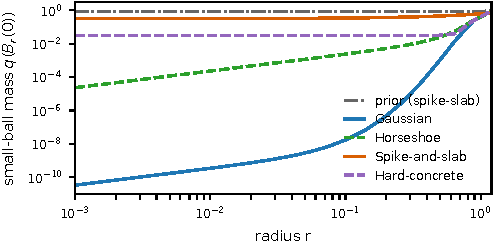
\includegraphics[width=\columnwidth,height=0.19\textheight,keepaspectratio]{results/figures/fig_nn_small_ball_cifar.pdf}
    \vspace{-0.4em}
    \caption{\color{blue} CIFAR-10 / ResNet-56 channel gates: per-channel small-ball mass.
    Continuous gates give $\MI_{\mathrm{pow}}=1$; atom-capable gates plateau at their
    channel-off atom ($\MI_{\mathrm{pow}}=\infty$). The legend entry ``Horseshoe'' is the
    mean-field Student-$t$ family of Experiment~4.}
    \label{fig:nn_sb_cifar}
    \vspace{-0.8em}
\end{figure}

\begin{figure}[t!]
    \centering
    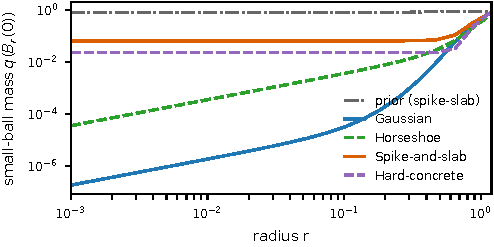
\includegraphics[width=\columnwidth,height=0.19\textheight,keepaspectratio]{results/figures/fig_nn_small_ball_imagenet.pdf}
    \vspace{-0.4em}
    \caption{\color{blue} ImageNet / ResNet-50 channel gates: per-channel small-ball mass,
    averaged over three seeds. The atom-capable gates plateau at their channel-off atom,
    giving $\MI_{\mathrm{pow}}=\infty$; the continuous gates decay with slope $1$. The
    legend entry ``Horseshoe'' is the mean-field Student-$t$ family of Experiment~4.}
    \label{fig:nn_sb_imagenet}
    \vspace{-0.8em}
\end{figure}

\begin{figure}[t!]
    \centering
    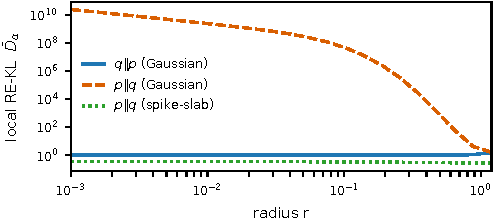
\includegraphics[width=\columnwidth,height=0.19\textheight,keepaspectratio]{results/figures/fig_nn_directional_rekl_cifar.pdf}
    \vspace{-0.4em}
    \caption{\color{blue} CIFAR-10 / ResNet-56 channel gates: directional local RE-KL. The
    $\pi_0\|q$ direction diverges for the continuous Gaussian gate (atom not matched) and
    stays bounded for the spike-and-slab gate.}
    \label{fig:nn_dir_cifar}
    \vspace{-0.8em}
\end{figure}

\begin{figure}[t!]
    \centering
    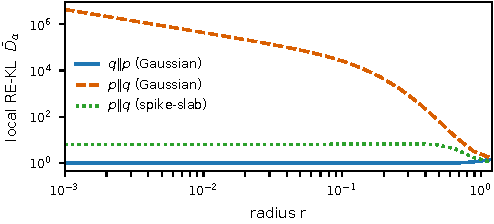
\includegraphics[width=\columnwidth,height=0.19\textheight,keepaspectratio]{results/figures/fig_nn_directional_rekl_imagenet.pdf}
    \vspace{-0.4em}
    \caption{\color{blue} ImageNet / ResNet-50 channel gates (trained on the frozen
    pretrained network), averaged over three seeds: the continuous-gate $\pi_0\|q$
    direction diverges as $r\downarrow0$, while the spike-and-slab gate remains bounded.
    As in Figure~\ref{fig:nn_dir_cifar}, the magnitude of the divergence reflects how
    tightly the continuous gate concentrates at the ``on'' value $1$.}
    \label{fig:nn_dir_imagenet}
    \vspace{-0.8em}
\end{figure}
